\chapter{MARCO TEÓRICO}
	\section{Geofísica y Geoeléctrica}
		\subsection{Definición de Geofísica}
			
			En términos generales la geofísica es la aplicación de los principios físicos de la materia en el estudio del planeta Tierra, o cual quier otro cuerpo celeste, desde el campo magnético, pasando por los fenómenos atmosféricos al medio solido del subsuelo, hasta las profundidades del núcleo interno planetario, ya sea que se empleé una fuente natural como la propagación de ondas elásticas generadas por sismicidad, ó bien, la inducción de campo electromagnético de fuente controlada \citep{parasnis2012, reynolds2011, lay1995}.   
		
			El  nacimiento de la geofísica es relativamente reciente, la primera prospección geoeléctrica data de 1830 realizados por \cite{fox1830} en Cornwal, Reino Unido, donde aplico técnicas de Self-Potential en exploración de mineralización de sulfuro en vetas, la medición del potencial natural resulto altamente efectiva para la prospección de este tipo de mineralizaciones ya que su anomalía se caracterizaba por presentar una respuesta muy marcada con respecto al medio \citep{reynolds2011, revil2013}.
			
		\subsection{Resistividad de la Tierra}
				
			De manera general la materia presenta características definidas a partir de los elementos que la integran, en primer orden la configuración atómica establece las propiedades físicas corresponden a la estructura de electrones, protones y neutrones que presentan los átomos; a su vez, las moléculas pueden estar conformadas por una clase especifica de átomos (moléculas homonucleares) o por conjuntos de diferentes tipos (compuestos), cuya conformación depende de factores físico-químicos \citep{tiab2024}.
			
			La configuración molecular inorgánica presente en la materia, definirá el tipo de estructura cristalina (mineral) que formarán, en conjunto; esta configuración cristalina es la que encontramos en el medio geológico conformando los minerales que componen la estructura mineral de una unidad geológica (ver figura \ref{fig:eo}) \citep{gandhi2016, tiab2024}.\\
			
			\begin{figure}[h!]
				\centering
				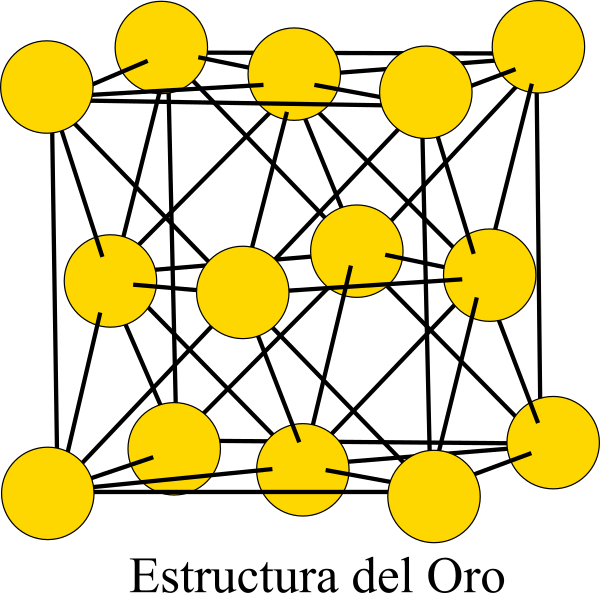
\includegraphics[width=9cm]{Imagenes/estructura-oro}
				\caption[Estructura atómica del oro]{Esquema de la estructura atómica de oro que conforma la cristalización octahedral, modificado de \citet{sorrell1973}}.
				\label{fig:eo}
			\end{figure}
			
			Los métodos Geoeléctricos se clasifican en dos grupos, métodos pasivos y de inducción, los primeros corresponden a aquellos en los que se mide el potencial eléctrico natural, usualmente medido en mili volts, en donde se requiere de electrodos no polarizables para tener medidas lo más claras posibles; mientras que los métodos de inducción emplean un arreglo de electrodos, o inductores de campo electromagnéticos, mediante los cuales se induce un campo eléctrico al subsuelo, calculando la diferencia de potencia eléctrica en el medio, o bien, el decaimiento de la polarización inducida \citep{revil2013, reynolds2011, igboama2023}.
			
			Los métodos de inducción, Sondeo Eléctrico Verticales (VES, por sus siglas en inglés), Tomografía de Resistividad Eléctrica (ERT, por sus siglas en inglés), Polarización Inducida (IP, por sus siglas en inglés), presentan una gran ventaja ya que no dependen del medio para poder realizar una lectura, ademas de poder realizarlos en cualquier momento, manteniendo el equipo en condiciones de operación, y pode diseñar arreglos de adquisición que nos permitan tener un muestreo tan amplio o limitado como sea conveniente, solo limitados por el alcance y potencia de los equipos empleados. Por otro lado su interpretación presenta un alta ambigüedad, solo acotado por la cantidad de referencias que puedan cruzarse para robustecer el modelo geológico y de inversión, y así poder llegar a una interpretación satisfactoria \citep{reynolds2011, igboama2023}.
			
			El método de prospección geoeléctrica, en especifico el SEV y la TRE, consiste en determinar la distribución de resistividades del subsuelo, de manera que se pueda establecer una correlación entre la resistividad y un modelo ajustado a la realidad geológica-estructural, geotécnica o geohidrológica del objeto de estudio.
	
		\subsection{Sondeo Eléctrico Vertical}
			
			Los SEV corresponden al método de mas rápida ejecución y económicamente mas accesible, por lo que es ampliamente empleado para solucionar problemas de ingeniería, minería, geotecnia, monitoreo e impacto ambiental y abastecimiento de Aguas potable; siendo de gran utilidad en la exploración de hidrogelogica ya que la respuesta resistiva de un medio saturado permite establecer diferencias concisas y discriminar entre agua dulce, salada, rocas fracturadas, arcillas , arenas, conglomerados, etc.
			
			La resistividad es medida mediante la inyección de una corriente en el subsuelo y mientras que se monitorea y captura la diferencia de potencial eléctrico en la superficie, esta lectura corresponde al valor de la contribución resistiva de todas las capas por donde fluye la corriente.
			
			La inyección de corriente y medición del potencial se realiza a través de un arreglo de dos pares de electrodos, $A, B (C_{1}, C_{2})$ y $M, N (P_{1}, P_{2}) $ respectivamente, siendo el electrodo $A (C_{1})$ el polo positivo y $B (C_{2})$ el polo negativo de inyección, mientras que el electrodo $M (P_{1})$ corresponde al polo positivo y $N (P_{2})$ al polo negativo de los electrodos de potencial.\\
			 
			\begin{figure}[h!]
				\centering
				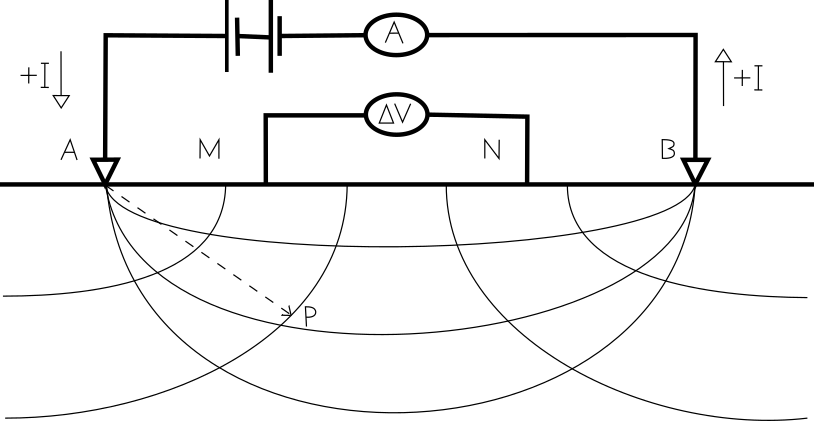
\includegraphics[width=9cm]{Imagenes/ArregloElectrodos}
				\caption[Configuración general de electrodos]{Configuración general de arreglo de electrodos, modificado de \citet{reynolds2011}}.
				\label{fig:AE}
			\end{figure}
			La resistividad del subsuelo se calcula a partir de la ley de Ohm, considerando el caso general en donde el medios es homogéneo y el arreglo de electrodos presenta una distribución convencional, donde se establece una relación directamente proporcional entre la la resistencia $R$ ,medida en Ohm ($\Omega$), y el cociente entre la diferencia de potencial $\Delta V$ y la corriente inducida $I$, para un valor puntual \citep{igboama2023}.
			
			\begin{equation}
				R = \frac{\Delta V}{I}
			\end{equation}
			   
			Sabiendo que se puede calcular $R$ para una sección con longitud $L$ y un área $A$, transversal del material, conociendo la resistividad ($\rho$) del material \citep{igboama2023, lowrie2020}, podemos reescribir la ecuación como: 
			
			\begin{equation}
				R = \rho \frac{L}{A}  \rightarrow  	\rho  = R \frac{A}{L} \rightarrow \rho  = R \cdot k
			\end{equation}
			
			Donde la resistividad ($\rho$) es una constante de proporcionalidad del medio y $k$ es el factor geométrico de distribución del flujo de corriente en términos de la del arreglo  de los electrodos de inducción y potencial (distancias entre los electrodos A-M-N-B ) \citep{igboama2023, lowrie2020}.
			
			\begin{equation}
				k = 2\pi \left(  \dfrac{1}{AM} - \dfrac{1}{AN} - \dfrac{1}{BM} + \dfrac{1}{BN} \right) 
			\end{equation}
			
			Tenemos que la resistividad aparente ($\rho _{A}$) de una sección del subsuelo, corresponde a la contribución resistiva de las unidades geológicas en esa sección, en términos de las distancias entre electrodos, la diferencia de potencial y el flujo de corriente en el medio \citep{igboama2023, lowrie2020}, esta dado por la siguiente ecuación:
			
			\begin{equation}
				\rho_{A} = \frac{\Delta U}{I} \cdot k %\rho_{A} = 2\pi \cdot \frac{\Delta U}{I} \cdot k
			\end{equation}
			
			\subsubsection{Arreglo de Electrodos y Factor Geométrico}
			
				Cada arreglo presenta ventas, desventajas, rango de sensibilidad y espacio de ejecución, debido a estas características y se tiene que evaluar e identificar que arreglo cumple con las condiciones adecuadas para ser ejecutado, considerando el espacio disponible en el sitio de estudio, el nivel de ruido (motores, conexiones a tierra mal aterrizadas, antenas, postes metálicos, arboles), la profundidad de objeto de prospección y la resolución vertical alcanzable (ver figura \ref{fig:Contri}).
				
					\begin{figure}[h!]
						\centering
						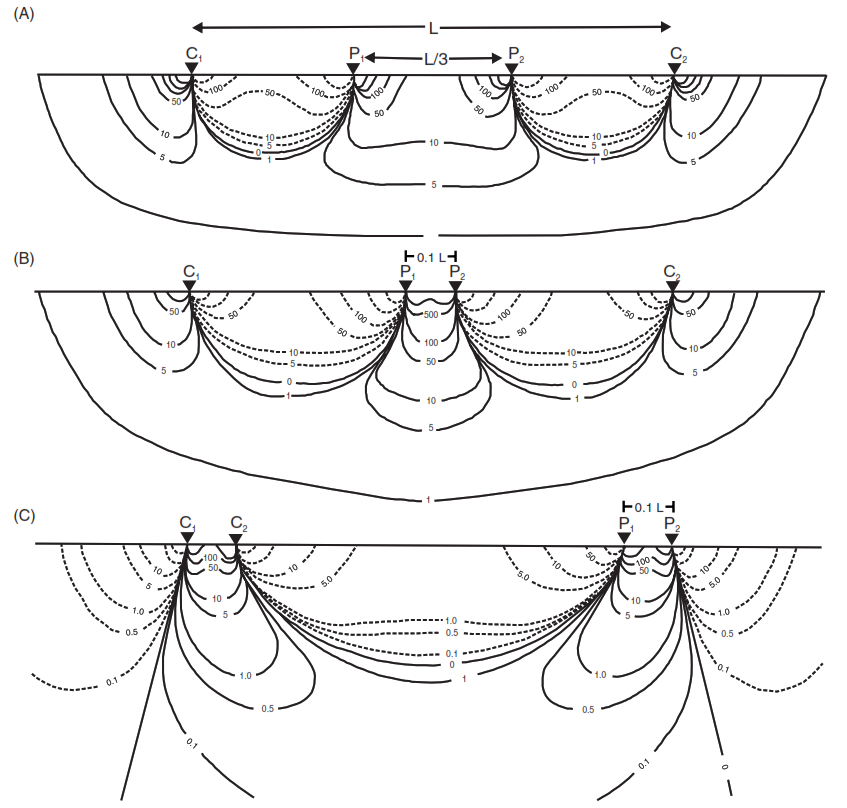
\includegraphics[width=12cm]{Imagenes/5}
						\caption[Esquema de la contribución de la respuesta eléctrica]{Esquema de la contribución de la respuesta de resistividad eléctrica, modificado de \citet{reynolds2011}}.
						\label{fig:Contri}
					\end{figure}				
				
				Como se observa en la sección anterior, la resistividad se determina empleando una configuración de los electrodos durante una medición, las distintas configuraciones de electrodos se encuentran ampliamente documentadas, cada una presenta un factor geométrico distinto \citep{igboama2023, lowrie2020}, los principales arreglos geoeléctricos son:
				
				\begin{description}
					\item[Wenner ]  
							\begin{equation}
								\rho_{A} = 2\pi \cdot R \cdot a
							\end{equation}
							
							\begin{figure}[h!]
								\centering
								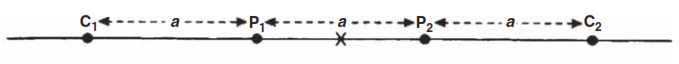
\includegraphics[width=9cm]{Imagenes/1}
								\caption[Esquema del arreglo Wenner]{Esquema del arreglo Wenner, modificado de \citet{reynolds2011}}.
								\label{fig:AW}
							\end{figure}
							
					\item[Schlumberger ] 
					
						\begin{equation}
							\rho_{A} = \frac{\pi a^{2}}{b} \left[ 1 - \frac{b^{2}}{4 a^{2}} \right] \cdot R, \quad a \geq 5b
						\end{equation}

							\begin{figure}[h!]
								\centering
								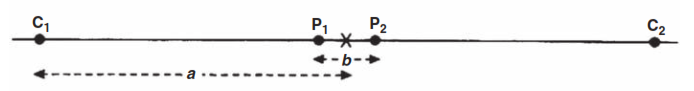
\includegraphics[width=9cm]{Imagenes/2}
								\caption[Esquema del arreglo Schlumberger]{Esquema del arreglo Schlumberger, modificado de \citet{reynolds2011}}.
								\label{fig:AS}
							\end{figure}
					
					\item[Dipolo-dipolo]  
					
							\begin{equation}
								\rho_{A} = \pi n(n+1)(n+2)a \cdot R
							\end{equation}
					
							\begin{figure}[h!]
								\centering
								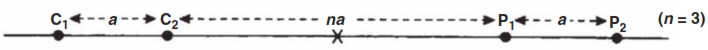
\includegraphics[width=9cm]{Imagenes/3}
								\caption[Esquema del arreglo Dipolo-dipolo]{Esquema del arreglo Dipolo-dipolo, modificado de \citet{reynolds2011}}.
								\label{fig:ADD}
							\end{figure}
				\end{description}
	
	\section{Adquisición de Datos Geofísicos}
	
	Previo al trabajo de adquisición se realiza un análisis de entorno, en el cual se verifica la viabilidad del arreglo dadas las condiciones del sitio, considerando lo siguiente: espacio disponible en el sitio de estudio, profundidad de exploración, nivel de ruido eléctrico, interferencias con la estabilidad del potencial natural del subsuelo, profundidad del objeto de exploración y dimensiones aproximadas del mismo.
	
		\subsection{Intervalo de Muestreo en SEV}
			
			El intervalo de muestreo empleado durante la adquisición de un SEV es un parámetro crítico que influye en la calidad y precisión de los datos geofísicos adquiridos, ya que esta estrechamente relacionado con la resolución vertical que deseamos de acuerdo al objeto de estudio. Durante la planeación es necesario considerar distintas condiciones, como son:
			
			\begin{itemize}
				\item Los espesores de cada unidad.
				\item La distribución de las distintas unidades.
				\item Profundidad de investigación
				\item Ruido en la señal.
			\end{itemize}
			
			Para establecer un intervalo de muestreo apropiado, se deben considerar el Teorema de Muestreo de Nyquist y El teorema de Shannon-Hartley (teorema de codificación de canal ruidoso)
			
			El Teorema de Muestreo de Nyquist, el cual, es un principio fundamental en el procesamiento de señales analógicas y digitales, donde establece las condiciones mínimas necesarias para una reconstrucción una señal analógica a partir de muestras discretas \citep{alvarado2010}.
			
			Nyquist nos garantiza las condiciones necesarias y suficientes para llevar a cabo una adquisición exitosa de muestreo de una señal, llámese distribución de resistividad en un medio heterogéneo y discontinuo \citep{alvarado2010}.
			
			\begin{equation}
				f_{s} \geq 2 \cdot f_{max}
			\end{equation}
			
			Donde la frecuencia de muestreo $f_{s}$ es por lo menos dos veces mayor a la frecuencia máxima $f_{max}$ conocida, cuando el teorema no se cumple se genera una distorsión en la señal, sumando las frecuencias altas incompletas a la señal natural de baja frecuencia, generando ruido, y problemas de interpretación, se conoce como aliasing \citep{alvarado2010}. 
			
			Considerando el medio geológico como una región con presencia coanstante de ruido electrico de fuentes tanto naturales como humanas, es impresindible considerar el teorema de Shannon-Hartley aplicando apilamiento de muestreo como metodo de reduccion de la relacion ruido señal, durante la adquisicion de datos; esto quiere decir calcular el promedio de muestreos cointinuos en un intervalo definido de aperturas entre electrodos.
			
			%% agregar ecuacion de shanon y desgrlosar sus elementos e interpretacion
				
			\subsubsection{Factores que Determinan el Intervalo de Muestreo}
		
				En el contexto de la adquisición de datos mediante SEV, el intervalo de muestreo es equivalente al espaciado entre puntos donde se realizan mediciones de resistividad del subsuelo. Este intervalo de muestreo debe ser lo mas pequeño posible, de modo que permita obtener muestras de resistividad \citep{telford1990}, esta relación se define de la siguiente manera:
				
				\begin{equation}
					f_{s}= \frac{1}{\Delta x}
				\end{equation}
				
				donde el intervalo de muestreo $\Delta x$ debe ser menor a la mitad de la longitud de onda ($\lambda_{min}$, espesor) asociado al objetivo de exploración
				
				\begin{equation}
					\Delta x \leq \frac{\lambda_{min} }{2}
				\end{equation}
				
				
			
		\subsection{Proceso de Adquisición In Situ}
			La adquisición de datos se realiza mediante la lectura directa en campo, al inducir corriente continua empleando un resistivimetro mediante de los electrodos de corriente A ($C_{1}$) y B ($C_{2}$), mientras se realiza la lectura de potencia en los electrodos M ($P_{1}$) y N ($P_{2}$), la lectura se realiza en intervalos regulares en instantes de inyección de corriente distintos \citep{telford1990}.
			
			Durante la toma de datos es importante considerar los modelos previos realizados durante el análisis preliminar, ya que las resistividades esperadas para las unidades, permiten tener control en la dispersión de datos, identificando tomas erróneas y corrigiendo al momento con una nueva lectura \citep{telford1990}.
	
	\section{Machine Learning (ML) en la Geofísica}  
	
	La aplicación de ML y el DL en la geofísica es ampliamente utilizado en exploración sísmica, abarcando los procesos de adquisición, procesado e interpretación, mejorando los tiempos de procesamiento, clasificación e interpretación, ya que es en este método donde se cuenta con la mayor cantidad de datos para entrenamiento \citep{wrona2018}; en menor medida se implementan técnicas de ML en la exploración y prospección geoeléctrica, hay algunos ejemplos destacables como son \cite{liu2020, el2001, li2024}, sin embargo no es un estándar en la industria, pese a las ventajas que puede tener su aplicación, como es el caso de este estudio
		
	El aprendizaje automático o machine learning, son un conjunto de técnicas que utilizan algoritmos con los cuales permite a un sistema aprender y generar predicciones, para lo que requiere un conjunto de datos para poder realizar el entrenamiento. Podemos clasificar los algoritmos de ML de dos maneras, por el tipo de aprendizaje, correspondiendo a Aprendizaje supervisado, no supervisado y por refuerzo, y por la relación que establecen con los parámetros del conjunto de datos de entrenamiento, es decir, modelos paramétricos y no paramétricos \citep{li2024}. 
	
	De los modelos no paramétricos destacan por su adaptabilidad a la estructura subyacente de los datos, por lo que pueden realizar aprendizaje de relaciones complejas entre datos, así como ausentes de linealidad, teniendo un costo en volumen de datos, requiriendo un número mayor para su entrenamiento, destacan los algoritmos siguientes.
	
	\begin{itemize}
		\item Árboles de decisión
		\item Random Forests
		\item K-Nearest Neighbors (KNN)
		\item Máquinas de soporte vectorial (kernelizados)
	\end{itemize}
	
	Dada la naturaleza de los datos de SEV's, heterogéneos, discontinuos y no lineales, es conveniente abordar su analistas desde un enfoque no paramétrico, teniendo esto en cuanta, la técnica Random Forests destaca siendo eficaz en la tarea de clasificación y regresión, teniendo algunos beneficios como son la reducción del sobre ajuste, interpretación de variables, resistencia al aliasing.
	
	\section{Random Forests} 
	
		La técnica Random Forests emplea múltiples arboles de decisión independientes entre si, donde cada árbol realiza una votación de clases, donde se selecciona la más popular de la entrada de cada árbol realizando una combinación de salida, permitiendo realizar una clasificación de características complejas o realizar regresiones de datos complejos multivariables \citep{breiman2001, lan2020}.
		
		La herramienta de Random Forests, de acuerdo con \citet{breiman2001} emplea tres elementos clave en el proceso de entrenamiento, bagging, selección aleatoria de características y agregación por votación, resultando en la combinación del los resultados en una predicción o clasificación robusta y ajustada \citep{lan2020}.
		
		\subsection{Siembra del bosque}
		
			\citet{breiman2001} nos dice que Random Forests es un conjunto de clasificadores $H(x,\theta_{k})$, $x$ es un vector de entrada y $\theta_{k}$ corresponden a vectores aleatorios independientes.
			
			A partir de los datos de entrada, se generan subconjuntos de datos de entrenamiento, estos se seleccionan con cierta aleatoriedad empleando la técnica bootstrap sampling, en cada nodo de los subconjuntos de entrenamiento se selecciona un subconjunto de características por votación de popularidad, dejando crecer cada árbol sin realizar poda hasta completar los criterios de finalización, es decir un numero de instancias preestablecido\citep{breiman2001}.
			
		\subsection{Predicciones del bosque}
		
			
			 La salida de un Random Forest para una entrada $x$ se basa en las predicciones individuales de los árboles para cada clase $h_{k}(x)$, se realiza un conteo de cada clase, producto de la predicción de cada árbol, sumando las salidas $I(h_{k}(x)=c)$, y finalmente se selecciona clase con mayor numero de predicciones, obteniendo la predicción de clasificación $H(x)$,donde $x$ es una función indicadora que vale 1 si $h_{k}(x)=c$, y $0$ en caso contrario \citep{breiman2001}.
			
			\begin{equation}
				H(x) = \text{argmax}_c \sum_{k=1}^K I(h_k(x) = c)
			\end{equation}

			
			El proceso de la regresión se obtiene a partir de la media aritmética de cada predicción individual, donde cada árbol produce un valor numérico $h_{k}(x)$ correspondiente a cada $x$, al corresponder con promedio de las predicciones se le otorga mas estabilidad cuando tenemos un numero elevado de arboles  y un conjunto de datos grande, entendiéndolo como un modelo central que incorpora información de cada árbol \citep{breiman2001}. 
			
			\begin{equation}
					H(x) = \frac{1}{K} \sum_{k=1}^K h_k(x)	
			\end{equation}

		\subsection{Margen y Error de Generalización}
		\subsection{Robustez y Convergencia}
		\subsection{Aplicaciones de Random Forests en Geofísica}
	